\begin{exo}{}
	Écrire sous forme d'intervalles les représentations graphiques suivantes :
	\begin{enumerate}
		\item
		      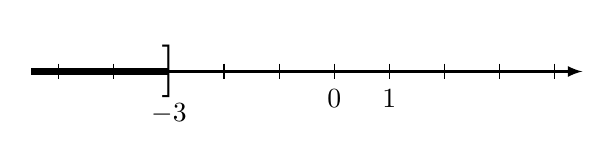
\begin{tikzpicture}[baseline=(current bounding box.center), scale=0.7, >=latex]
			      \draw[->, thick] (-5.5,0) -- (4.5,0);
			      \foreach \x in {-5,-4,-3,-2,-1,0,1,2,3,4} \draw (\x,4pt) -- (\x,-4pt);
			      \node[below=1pt] at (0,-0.1) {$0$};
			      \node[below=1pt] at (1,-0.10) {$1$};
			      \node[below=6pt] at (-3,-0.10) {$-3$};
			      \draw[ultra thick, line width=2.5pt] (-5.5,0) -- (-3,0);
			      \node[thick, scale=1.9, text=black] at (-3,0) {$]$};
		      \end{tikzpicture}

		\item
		      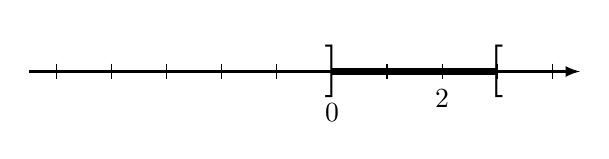
\begin{tikzpicture}[baseline=(current bounding box.center), scale=0.7, >=latex]
			      \draw[->, thick] (-5.5,0) -- (4.5,0);
			      \foreach \x in {-5,-4,-3,-2,-1,0,1,2,3,4} \draw (\x,4pt) -- (\x,-4pt);
			      \node[below=6pt] at (0,-0.10) {$0$};
			      \node[below=1pt] at (2,-0.10) {$2$};
			      \draw[ultra thick, line width=2.5pt] (0,0) -- (3,0);
			      \node[thick, scale=1.9, text=black] at (0,0) {$]$};
			      \node[thick, scale=1.9, text=black] at (3,0) {$[$};
		      \end{tikzpicture}

		\item
		      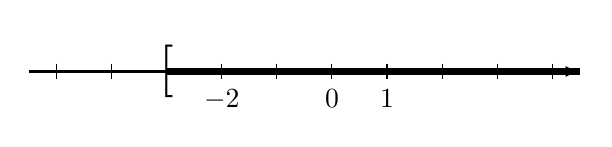
\begin{tikzpicture}[baseline=(current bounding box.center), scale=0.7, >=latex]
			      \draw[->, thick] (-5.5,0) -- (4.5,0);
			      \foreach \x in {-5,-4,-3,-2,-1,0,1,2,3,4} \draw (\x,4pt) -- (\x,-4pt);
			      \node[below=1pt] at (0,-0.10) {$0$};
			      \node[below=1pt] at (1,-0.10) {$1$};
			      \node[below=1pt] at (-2,-0.10) {$-2$};
			      \draw[ultra thick, line width=2.5pt] (-3,0) -- (4.5,0);
			      \node[thick, scale=1.9, text=black] at (-3,0) {$[$};
		      \end{tikzpicture}
	\end{enumerate}
\end{exo}
